\section{Sliding Windows and Data Parallelization}

\begin{figure}[t]
\centering
\begin{subfloat}
\begin{minipage}[b]{0.45\textwidth}
\eightpoint
\begin{verbatim}
float->float filter FIR(int N) {
  int srcBuffer[N];
  int srcEnd = 0; 
  ...
  work push 1 pop 1 {
    srcBuffer[srcEnd] = pop();
    float sum = 0;
    for (int i=0; i<N; i++) {
      sum += weights[i] * srcBuffer[(srcEnd + i + 1) % N];
    }
    push(sum);
    srcEnd = (srcEnd + 1) % N;
  }
}
\end{verbatim}
\vspace{-8pt}
\end{minipage}%
\caption{ \label{fig:fir-nopeeking}}
\end{subfloat}%
\qquad
\begin{subfloat}
\begin{minipage}[b]{0.45\textwidth}
\eightpoint
\begin{verbatim}
float->float filter FIR(int N) {
  ...
  work push 1 pop 1 peek N {
    float sum = 0;
    for (int i=0; i<N; i++) {
      sum += weights[i] * peek(i);
    }
    push(sum);
    pop();
  }
}
\end{verbatim}
\vspace{-18pt}
\end{minipage}
\caption{ \label{fig:fir-streamit}}
\end{subfloat}
\caption[Two implementations of an FIR filter.]{\label{fig:fir-code}
  Two StreamIt implementations of an FIR filter:
   \subref{fig:fir-nopeeking} the non-peeking version implemented via a
  stateful circular buffer; and \subref{fig:fir-streamit} the peeking version. Only steady-state implementation is
  given.}
\end{figure}

For sliding window filters, some (or all) input items are required by
multiple iterations.  Without explicit support for sliding window
computations, shared items must be manually saved for a later
iteration.  Figure~\ref{fig:fir-nopeeking} gives an implementation of
an FIR filter in the StreamIt programming language without using the
language's peeking support.  This implementation requires
sophisticated compiler analyses in order to parallelize.
The programmer is forced to use a circular buffer to represent the
sliding window of the FIR computation.  Modulo operations are used in
the address calculation for the circular buffer.  Modulo operations
are typically not handled by array dependence analysis frameworks.  So
in the presence of modulo operations, the compiler must conservatively
assume that each read and write can access any location in the array.

Obscuring the data parallelism in sliding window computations limits
parallelization scalability.  For our benchmarks, ChannelVocoder,
Filterbank, and FMRadio, stateful implementations of sliding window
filters limits scalability to 18, 37, and 14 cores, respectively.
Figure~\ref{fig:fir-streamit} gives an implementation of an FIR filter
that utilizes StreamIt's peeking idiom.  The behavior of the sliding
window is described by the pop and peek rates.  The window is accessed
via the {\tt peek(i)} expression.  Exposing sliding windows in this
manner enables the techniques presented in this paper thus enabling
scalable parallelization to at least 64-cores.


\begin{figure}[t]
\centering
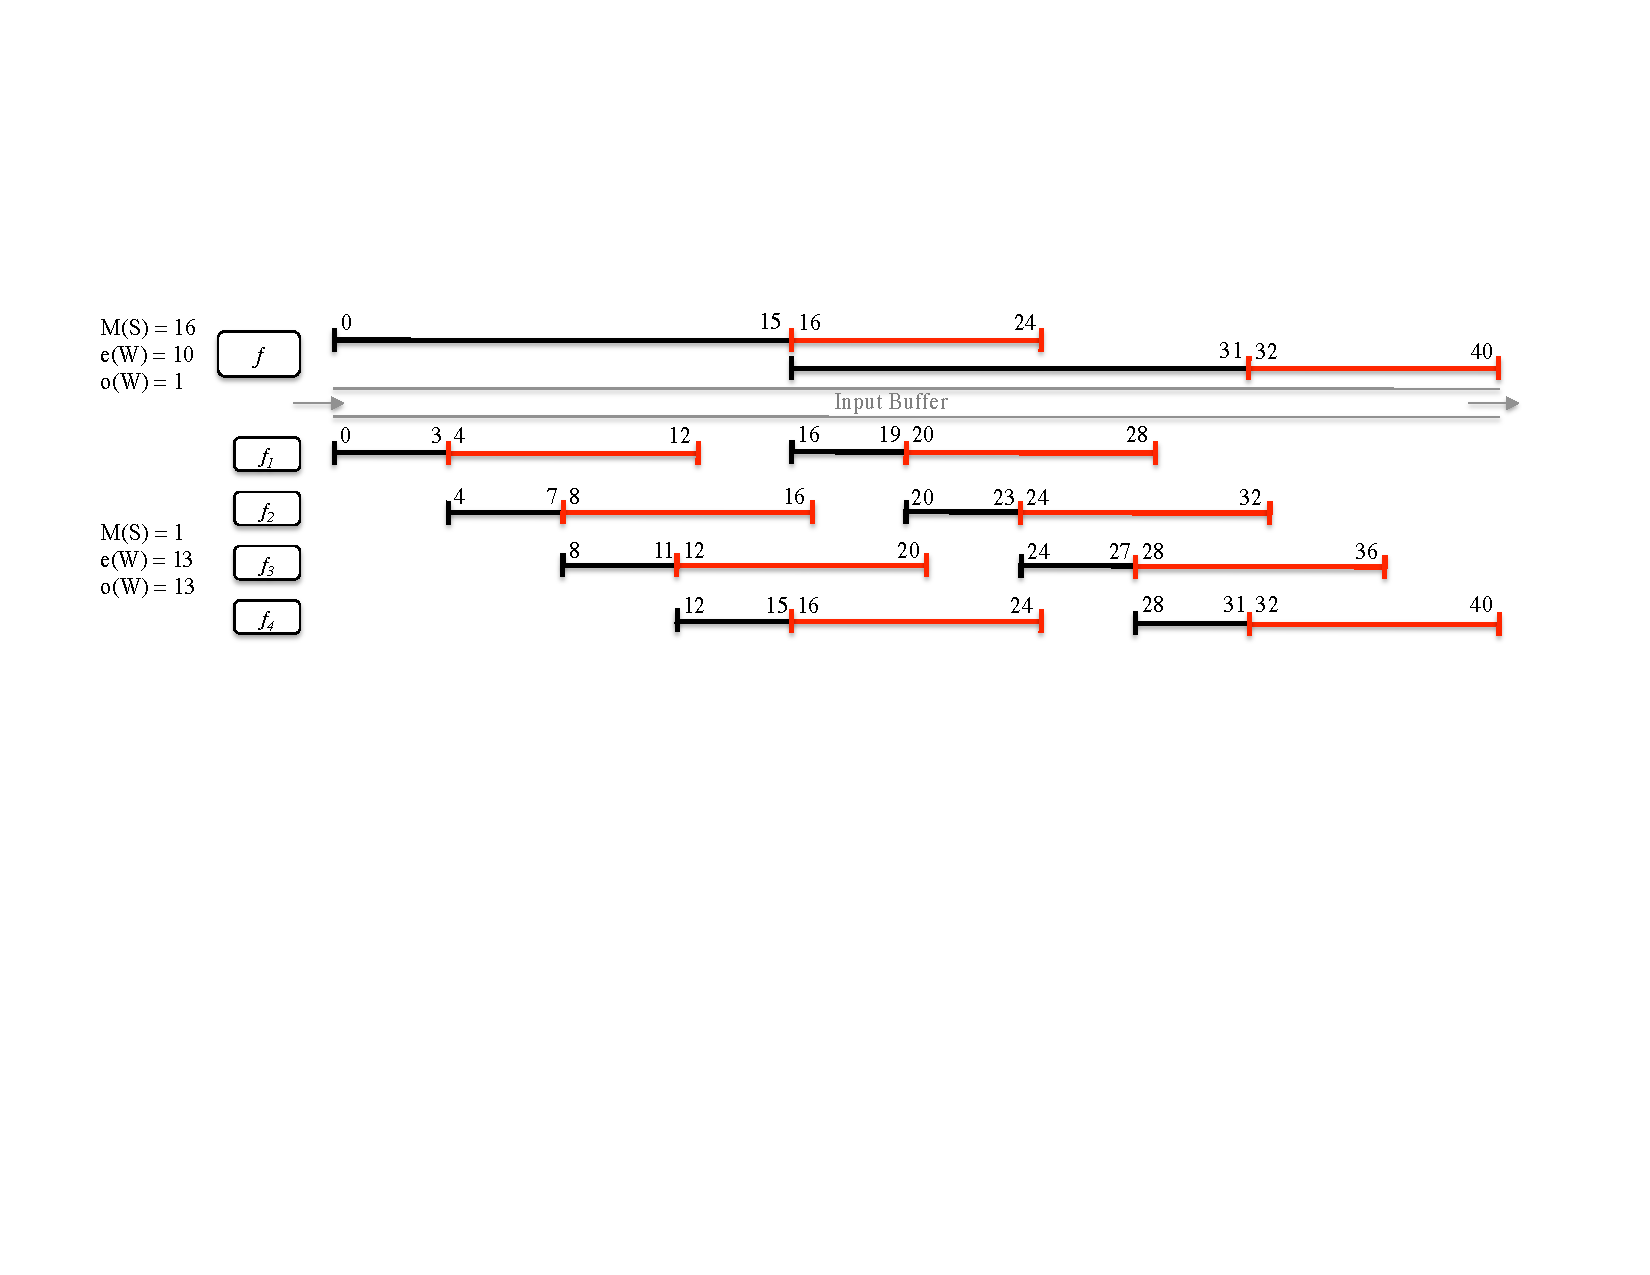
\includegraphics[width=3.0in]{figures/fission-sharing.pdf}
\caption[An example of the sharing required by fission.]  { An
  example of the duplication of items required by fission.  Filter $f$
  is fissed by 4 into $f_1$ - $f_4$.  Two steady-states of the item
  indices required for both $f$ and the fission products are shown.
  Item indices that are inspected but not dequeued are in red.  For the
  fission products, it is required to duplicate 1 out of 4 items to
  all 4 filters, and the remaining 3 items are duplicated to 3
  filters.  Notice that the number of items inspected by the fission
  products is the same as $f$, but the total number of items dequeued 
per steady-state is split across the $f_i$s.
\label{fig:fission-sharing}}
\end{figure}

Data parallelization is possible if the compiler can reason about the
sharing requirement of the sliding window filter.  When a sliding
window filter is parallelized via the process of fission, the window
state inherent between iterations is transformed into the
communication of shared items to multiple products of the filter.
Figure~\ref{fig:fission-sharing} gives an example of the sharing
requirement between fission products for a fission application. 
Previous work implement fission of sliding window filters via
duplication of all input items to all fission products and decimation
of unneeded items at each product filter~\cite{streamit-asplos}.  We
call this technique {\it DupDec}. If each product is mapped to a
distinct core, the replication of items is achieved via the
communication network.

The efficiency of DupDec depends on the application being mapped and
the communication mechanism of the target. For our benchmarks, we can
determine what percentage of total steady-state communication is
unnecessarily duplicated by DupDec guided by the techniques described
in~\cite{gordon-asplos06}:

\begin{itemize}
\item ChannelVocoder: 38\% unnecessarily duplicated (5,200 of 13,336
      total items)
\item FMRadio: 61\% unnecessarily duplicated (1,108 of
      1,808 total items) 
\item FilterBank: 0\% duplicated (912 total items)
\end{itemize}

Our techniques will always avoid unncessary duplication of input
items.  Even without unnecessarily duplication of items, inter-core
communication as a result of fission accounts for a large percentage
of the total items communicated between filters of an application.
ChannelVocoder has 48\% of total communication as inter-core
communication caused by fission, Filterbank 50\%, and FMRadio 93\%.
Employing our techniques, for our benchmarks, we are able to reduce
the percentage of inter-core communication by altering the steady
state.

In the general case, when fissing a filter that peeks, i.e., a filter
$f$ with $e(W, f) - o(W, f) = \mt{dup}_f < C(f) > 0$, by $P$, the producers
of $f$ need to duplicate output items to an average of:

\[ \max \left ( 1 + \frac{C(f)}{M(S, f) \cdot o(W, f) / P}, P \right )\]

\noindent fission products of $f$.  Figure~\ref{fig:fission-sharing}
gives an example of the required sharing for a fission application.
The filter $f$ is duplicated 4 ways, has $C(f) = 9$, $o(W, F) = 4$,
and $M(S, f) = 16$.  From the above formula, each item is duplicated
to an average of $3.25$ fission products.
